\begin{frame}
  \frametitle{Charm++ File structure}
  \begin{itemize}
    \item C++ objects (including Charm++ objects)
      \begin{itemize}
      \item Defined in regular \texttt{.h} and \texttt{.C} files
      \end{itemize}
    \item Chare objects, entry methods (asynchronous methods)
      \begin{itemize}
      \item Defined in \texttt{.ci} file
      \item Implemented in the \texttt{.C} file
      \end{itemize}
  \end{itemize}
  \begin{center}
    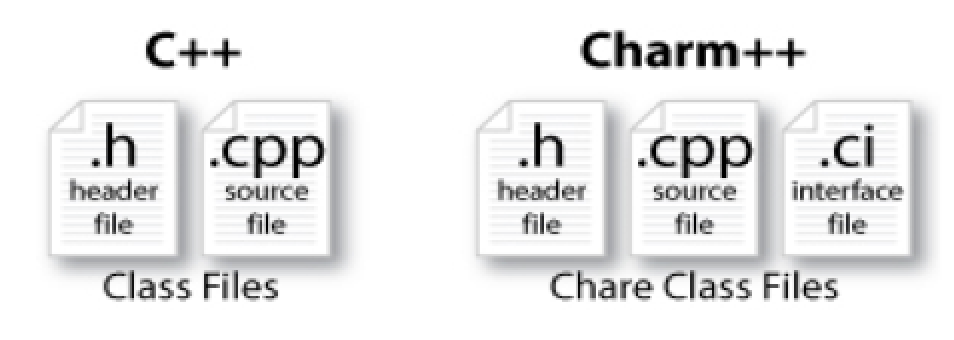
\includegraphics[width=0.6\textwidth]{figures/charmFiles.png}
  \end{center}
\end{frame}

\begin{frame}[fragile]
  \frametitle{Charm Interface: Modules}
  \begin{itemize}
    \item Charm++ programs are organized as a collection of modules
    \item Each module has one or more chares
    \item The module that contains the \textit{mainchare}, is declared as the
      \texttt{mainmodule}
    \item Each module, when compiled, generates two files:
      \code{MyModule.decl.h} and \code{MyModule.def.h}
  \end{itemize}
  \begin{center}
  \texttt{.ci file}
  \begin{lstlisting}
    [main]module MyModule {
      //... chare definitions ...
    };
  \end{lstlisting}
  \end{center}
\end{frame}

\begin{frame}[fragile]
  \frametitle{Charm Interface: Chares}
  \begin{itemize}
    \item Chares are parallel objects that are managed by the RTS
    \item Each chare has a set \textit{entry methods}, which are asynchronous
      methods that may be invoked remotely
    \item The following code, when compiled, generates a C++ class
      \code{CBase\_MyChare} that encapsulates the RTS object
    \item This generated class is extended and implemented in the \texttt{.C}
      file
  \end{itemize}
  \texttt{.ci file}
  \begin{lstlisting}
    [main]chare MyChare {
      //... entry method definitions ...
    };
  \end{lstlisting}
  \texttt{.C file}
  \begin{lstlisting}
    class MyChare : public CBase_MyChare {
      //... entry method implementations ...
    };
  \end{lstlisting}
\end{frame}

\begin{frame}[fragile]
  \frametitle{Charm Interface: Entry Methods}
  \begin{itemize}
  \item Entry methods are C++ methods that can be remotely and asynchronously
    invoked by another chare
  \end{itemize}
  \texttt{.ci} file:
  \begin{lstlisting}
    entry MyChare(); /* constructor entry method */
    entry void foo();
    entry void bar(int param);
  \end{lstlisting}
  \texttt{.C} file:
  \begin{lstlisting}
    MyChare::MyChare() { /*... constructor code ...*/ }

    MyChare::foo() { /*... code to execute ...*/ }

    MyChare::bar(int param) { /*... code to execute ...*/ }
  \end{lstlisting}
\end{frame}

\begin{frame}[fragile]
   \frametitle{Charm Interface: \texttt{mainchare}}
   \begin{itemize}
     \item Execution begins with the \texttt{mainchare}'s constructor
     \item The \texttt{mainchare}'s constructor takes a pointer to
       system-defined class \code{CkArgMsg}
     \item \code{CkArgMsg} contains \code{argv} and \code{argc}
     \item The \texttt{mainchare} will typically creates some additional chares
   \end{itemize}
\end{frame}

\begin{frame}[fragile]
  \frametitle{Creating a Chare}
  \begin{itemize}
    \item A chare declared as \code{chare MyChare \{...\};} can be
      instantiated by the following call:
  \end{itemize}
\begin{lstlisting}
CProxy_MyChare::ckNew(... constructor arguments ...);
\end{lstlisting}
  \begin{itemize}
  \item To communicate with this class in the future, a \textit{proxy} to it
    must be retained
  \end{itemize}
\begin{lstlisting}
CProxy_MyChare proxy = 
  CProxy_MyChare::ckNew(... constructor arguments ...);
\end{lstlisting}
\end{frame}

\begin{frame}[fragile]
  \frametitle{Chare Proxies}
  \begin{itemize}
  \item A chare's own proxy can be obtained through a special variable
    \code{thisProxy}
  \item Chare proxies can also be passed so chares can learn about others
  \item In this snippet, \code{MyChare} learns about a chare instance
    \code{main}, and then invokes a method on it:
  \end{itemize}
\texttt{.ci} file
\begin{lstlisting}
entry void foobar2(CProxy_Main main);
\end{lstlisting}
\texttt{.C} file
\begin{lstlisting}
MyChare::foobar2(CProxy_Main main) {
  main.foo();
}
\end{lstlisting}
\end{frame}

\begin{frame}[fragile]
   \frametitle{Charm Termination}
   \begin{itemize}
   \item There is a special system call \code{CkExit()} that terminates the
     parallel execution on all processors (but it is called on one processor)
     and performs the requisite cleanup
   \item The traditional \code{exit()} is insufficient because it only
     terminates one process, not the entire parallel job (and will cause a
     hang)
   \item \code{CkExit()} should be called when you can safely terminate the
     application (you may want to synchronize before calling this)
   \end{itemize}
\end{frame}

\begin{frame}
   \frametitle{Compiling a Charm++ Program}
   \begin{center}
     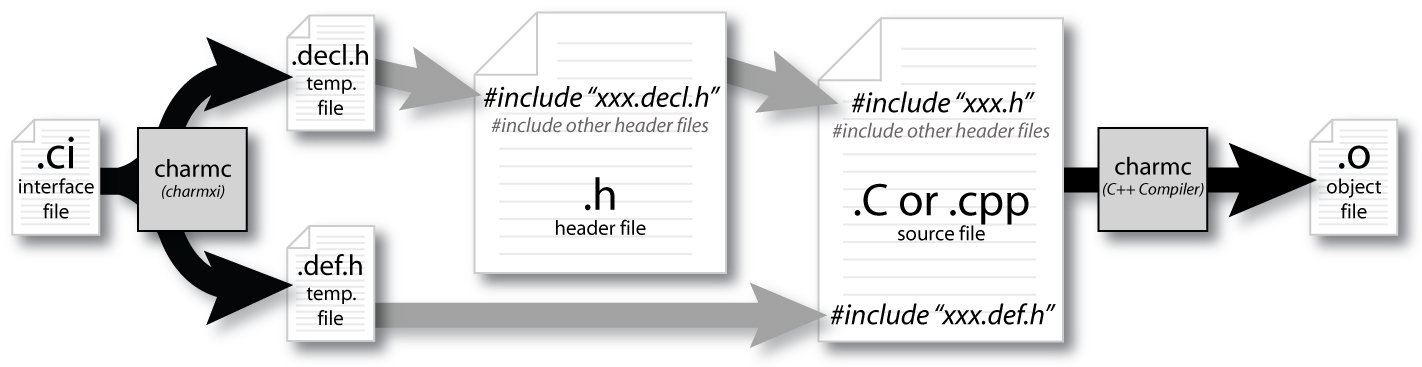
\includegraphics[width=0.9\textwidth]{figures/charmCompile.jpg}
   \end{center}
\end{frame}

\begin{frame}
  \frametitle{Building Charm++}
  \begin{itemize}
  \item git clone -b charm-6.5 git://charm.cs.uiuc.edu/charm.git
  \item ./build $<$TARGET$>$ $<$ARCH$>$ $<$OPTS$>$
  \item TARGET = Charm++, AMPI, bgampi, LIBS etc.
  \item ARCH = net-linux-x86\_64, pamilrts-bluegeneq etc.
  \item OPTS = --with-production, --enable-tracing, xlc, smp, -j8 etc.
  \item http://charm.cs.illinois.edu/manuals/html/charm++/A.html
  \end{itemize}
\end{frame}

\begin{frame}
  \frametitle{Hello World Example}
  \begin{itemize}
    \item Compiling
      \begin{itemize}
      \item \texttt{charmc hello.ci}
      \item \texttt{charmc -c hello.C}
      \item \texttt{charmc -o hello hello.o}
      \end{itemize}
    \item Running
      \begin{itemize}
      \item \texttt{./charmrun +p7 ./hello}
      \item The \texttt{+p7} tells the system to use seven cores
      \end{itemize}
    \end{itemize}
\end{frame}


\begin{frame}[fragile]
  \frametitle{Chare Creation Example: \texttt{.ci} file}
  \lstinputlisting{code/chareCreate.ci}
\end{frame}

\begin{frame}[fragile]
  \frametitle{Chare Creation Example: \texttt{.C} file}
  \lstinputlisting[basicstyle=\footnotesize]{code/chareCreate.C}
\end{frame}

\begin{frame}[fragile]
  \frametitle{Asynchronous Methods}
  \begin{itemize}
  \item Entry methods are invoked by performing a C++ method call on a chare's
    proxy
  \end{itemize}
  \begin{lstlisting}
CProxy_MyChare proxy =
  CProxy_MyChare::ckNew(... constructor arguments ...);

proxy.foo();
proxy.bar(5);
\end{lstlisting}
\begin{itemize}
\item The \code{foo} and \code{bar} methods will then be executed with the
  arguments, wherever the created chare, \texttt{MyChare}, happens to live
\item The policy is one-at-a-time scheduling (that is, one entry method on one
  chare executes on a processor at a time)
\end{itemize}
\end{frame}

\begin{frame}[fragile]
  \frametitle{Asynchronous Methods}
  \begin{itemize}
  \item Method invocation is not ordered (between chares, entry methods on one
    chare, etc.)!
  \item For example, if a chare executes this code:
  \begin{lstlisting}
CProxy_MyChare proxy = CProxy_MyChare::ckNew();
proxy.foo();
proxy.bar(5);
  \end{lstlisting}
  \item These prints may occur in \textbf{any} order
  \begin{lstlisting}
MyChare::foo() {
  ckout << "foo executes" << endl;
}

MyChare::bar(int param) {
  ckout << "bar executes with " << param << endl;
}
\end{lstlisting}
  \end{itemize}
\end{frame}

\begin{frame}[fragile]
  \frametitle{Asynchronous Methods}
  \begin{itemize}
  \item For example, if a chare invokes the same entry method twice:
  \begin{lstlisting}
proxy.bar(7);
proxy.bar(5);
  \end{lstlisting}%
  \item These may be delivered in \textbf{any} order
  \begin{lstlisting}
MyChare::bar(int param) {
  ckout << "bar executes with " << param << endl;
}
\end{lstlisting}
  \item Output
\begin{lstlisting}
bar executes with 5
bar executes with 7
\end{lstlisting}
\textbf{OR}
\begin{lstlisting}
bar executes with 7
bar executes with 5
\end{lstlisting}
  \end{itemize}
\end{frame}


\begin{frame}[fragile]
  \frametitle{Asynchronous Example: \texttt{.ci} file}
\begin{lstlisting}
mainmodule MyModule {
  mainchare Main {
    entry Main(CkArgMsg *m);
  };
  chare Simple {
    entry Simple(double y);
    entry void findArea(int radius, bool done);
  };
};
\end{lstlisting}
\end{frame}

\begin{frame}[fragile]
  \frametitle{Asynchronous Example: \texttt{.C} file}
\begin{itemize}
  \item Does this program execute correctly?
\end{itemize}
\scriptsize
\begin{lstlisting}[basicstyle=\footnotesize]
struct Main : public CBase_Main {
  Main(CkArgMsg* m) {
    double pi = 3.1415;
    CProxy_Simple sim =  CProxy_Simple::ckNew(pi);
    for (int i = 1; i< 10; i++) sim.findArea(i, false);
    sim.findArea(10, true);
  };
};

struct Simple : public CBase_Simple {
 float y;
 Simple(double pi) {
   y = pi;
   ckout << "Hello from a simple chare running on " << CkMyPe() << endl;
 }
 void findArea(int r, bool done) {
   ckout << "Area of a circle of radius" << r << " is " << y*r*r << endl;
   if (done) CkExit();
 }
};
\end{lstlisting}
\end{frame}

\begin{frame}[fragile]
  \frametitle{Data types and entry methods}
\begin{itemize}
  \item You can pass basic C++ types to entry methods (\texttt{int},
    \texttt{char}, \texttt{bool}, etc.)
  \item C++ STL data structures can be passed by including \texttt{pup\_stl.h}
  \item Arrays of basic data types can also be passed like this:\\
  \item \texttt{.ci} file:
\begin{lstlisting}
entry void foobar(int length, int data[length]);
\end{lstlisting}
  \item \texttt{.C} file:
\begin{lstlisting}
MyChare::foobar(int length, int* data) {
 // ... foobar code ...
}
\end{lstlisting}
\end{itemize}
\end{frame}

\begin{frame}[fragile]
  \frametitle{Readonlys}
  \begin{itemize}
  \item A \textit{readonly} is a global (within a module) read-only variable
    that can only be written to in the \texttt{mainchare}'s constructor
  \item Can then be read (\textbf{not written!}) by any chare in the module
  \item It is declared in the \texttt{.ci} file:
  \begin{lstlisting}
  readonly <type> <name>;
  readonly CProxy_Main mainProxy;
  readonly int numChares;
  \end{lstlisting}
  \item And defined the the \texttt{.C} file:
  \begin{lstlisting}
  <type> <name>;
  CProxy_Main mainProxy;
  int numChares;
  \end{lstlisting}
  \item And set in the \texttt{mainchare}'s constructor
  \begin{lstlisting}
  MyChare::MyChare(CkArgMsg *m) {
    mainProxy = thisProxy;
    numChares = 10;
  }
\end{lstlisting}


\end{itemize}
\end{frame}

\eat{
\begin{frame}[fragile]
  \frametitle{PI Example}
  \lstinputlisting{code/pi.ci}  
\end{frame}

\begin{frame}[fragile]
  \frametitle{PI Example}
  \lstinputlisting[basicstyle=\tiny]{code/piMaster.C}
\end{frame}

\begin{frame}[fragile]
  \frametitle{PI Example}
  \lstinputlisting{code/piWorker.C}
\end{frame}
}


